\section{Why location matters: a linear-Gaussian account}\label{sec:theory}
Let a frozen encoder yield a disease block with class-separation signal-to-noise ratio $S$ and an artifact block with
SNR $A$ per unit of artifact presence; training uses $P(A{=}1\mid Y{=}1)=p_1$, $P(A{=}1\mid Y{=}0)=p_0$ and the
reversed test swaps them. For the LDA-optimal linear head the artifact's effective training SNR is
$\tilde A=(p_1-p_0)^2A/(1+p_1(1-p_1)A)$ and
\begin{equation}
\mathrm{AUROC}_{\mathrm{rev}}(S,\tilde A)=\Phi\!\left(\frac{S-\tilde A}{\sqrt{2(S+\tilde A)}}\right),
\end{equation}
increasing in $S$ and decreasing in $\tilde A$ (verified by simulation to within 0.009 AUROC; Fig.~\ref{fig:theory}).
Masking maps $(S,\tilde A)\mapsto(S_m,\tilde A_m)$. Out of the ROI, $\tilde A_m=0$; inside, $\tilde A_m\ge\tilde A$.
Hence (i) in-ROI masking harms exactly when the mask removes disease-informative context ($S_m<S$) and helps only by
denoising ($S_m>S$); (ii) for any $S_m$ the benefit of masking is larger out of the ROI than inside it---the crossover
is always positive; (iii) erasing a subspace that contains the artifact direction sets $\tilde A\to0$ but scales $S$
by $1-\rho^2$, where $\rho$ is its overlap with the disease direction, so erasure beats in-ROI masking unless the
artifact resembles the pathology, which disease protection prevents; (iv) group balancing removes the
artifact--label association and everything correlated with it, giving $\Phi(\sqrt{S/2})$ irrespective of location;
(v) a shortcut carried by correlates that neither the mask nor pixel-level erasure touch can only be removed by
label-based reweighting. Each consequence is borne out in Sections~\ref{sec:derm}--\ref{sec:solution}.
\begin{figure}[t]\centering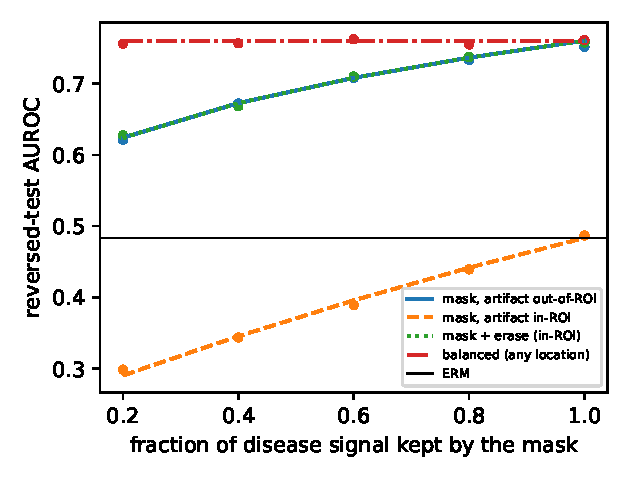
\includegraphics[width=0.6\linewidth]{figures/theory.pdf}
\caption{Reversed-test AUROC predicted by the linear-Gaussian model (lines) and simulated with logistic heads
(points) as masking removes a growing share of disease signal ($S=1$, $A=2$, 90/10 training). Generated by
\texttt{scripts/analysis/theory\_sim.py}.}\label{fig:theory}\end{figure}

\paragraph{Does the account match real encoders?} For any test composition $q_y=P(A{=}1\mid Y{=}y)$ the same head
gives $\mathrm{AUROC}=\Phi\big(\Delta/\sqrt{\sigma_1^2+\sigma_0^2}\big)$ with $\Delta=S+(p_1-p_0)(q_1-q_0)A/(1+vA)$,
$\sigma_y^2=S+w_a^2\,(1+Aq_y(1-q_y))$, $w_a=\sqrt{A}(p_1-p_0)/(1+vA)$ and $v=[p_1(1-p_1)+p_0(1-p_0)]/2$. In a
pre-registered test we fitted $(S,A)$ for every trained model to its clean and correlated AUROC \emph{only} and
compared the implied reversed-test AUROC with the held-out observation; no parameter is shared across models or tuned
(Fig.~\ref{fig:theory_predict}). Over 148 ERM and masking models (real traps, chest drains, controlled sweeps) the mean
absolute error is 0.039 AUROC ($r=0.92$), against 0.234 for ``reversed $=$ clean'' and 0.108 for a linear-symmetry
heuristic ($2\cdot$clean $-$ correlated). The implied location crossover agrees with the observed one across 14
cohort--backbone pairs ($r=0.997$, mean absolute error 0.014, 13/14 signs; the miss is a chest-radiograph cell with
an observed crossover of $-0.002$), the implied mask gains agree with the controlled sweeps ($r=0.965$, 42/45 signs),
and the agreement extends to end-to-end fine-tuned networks (4/4 crossover signs), which violate the model's
assumptions. Because our pre-registered criterion required every crossover sign to agree, we still call the model a
qualitative account. Its one clear failure is the chest-drain cohort (implied 0.70--0.76, observed 0.19--0.24): the
clean and correlated environments do not expose a shortcut carried by correlates of the drain, regime~(v).
\ifdupfloats
\begin{figure}[t]\centering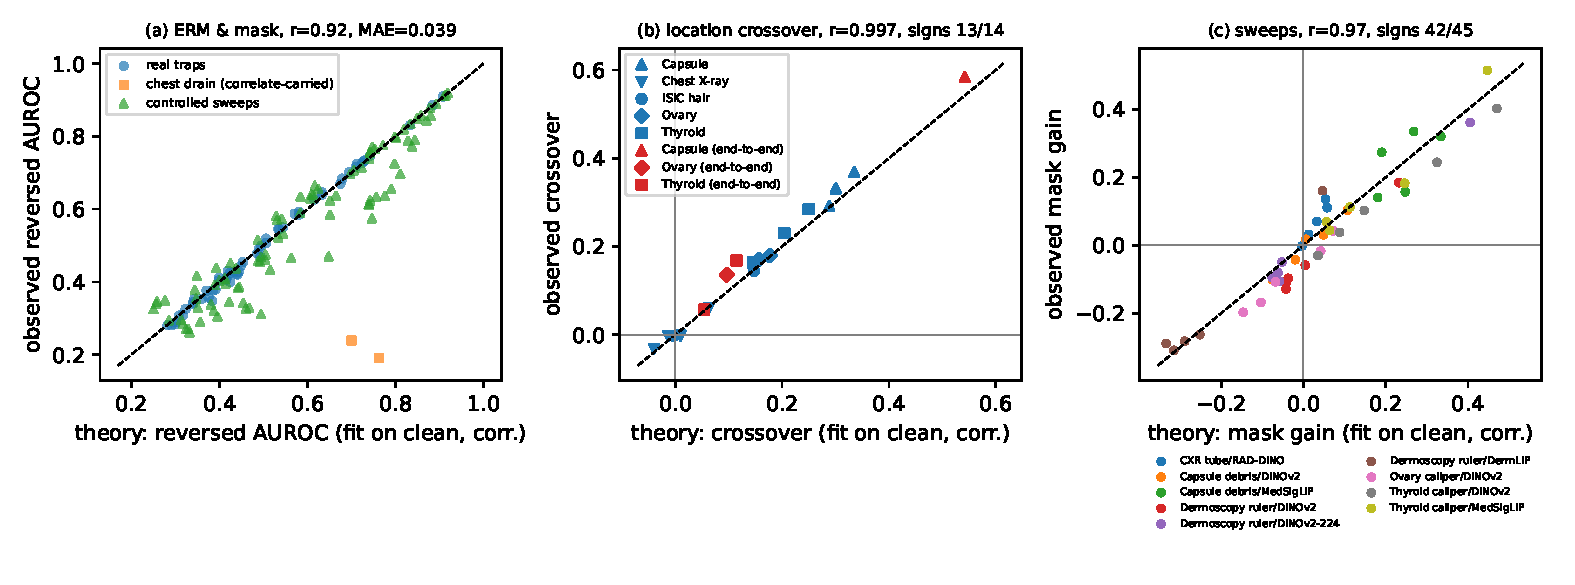
\includegraphics[width=\linewidth]{figures/theory_predict.pdf}
\caption{Pre-registered test of the linear-Gaussian account on real encoders. $(S,A)$ are fitted to each model's
clean and correlated AUROC; the reversed-test results are held out. (a) Implied vs observed reversed-test AUROC (ERM
and masking). (b) Location crossover per cohort and backbone; red: end-to-end fine-tuned networks, outside the
model's assumptions. (c) Mask $-$ ERM gain along the controlled overlap sweeps. Dashed: identity. Generated by
\texttt{scripts/analysis/theory\_predict.py}.}\label{fig:theory_predict}\end{figure}
\fi
